\chapter{Results}
\label{chap:results}

This chapter presents solutions to the ionosphere surface equation (Equation~\ref{eqn:continuity_eqn}) over seasonal and geomagnetic variation. All solves use the MueLu-preconditioned GMRES solver that was discussed in Section~\ref{sec:convergence_analysis}. Since the magnetosphere-ionosphere coupling is still in progress, these plots present the results of a single southward IMF source term that was provided by the magnetosphere model and interpolation used in~\citet{global_groth_2000}. Figure~\ref{fig:sourceTerm} shows the source term that was used in this analysis.
\begin{figure}[htbp]
	\centering
	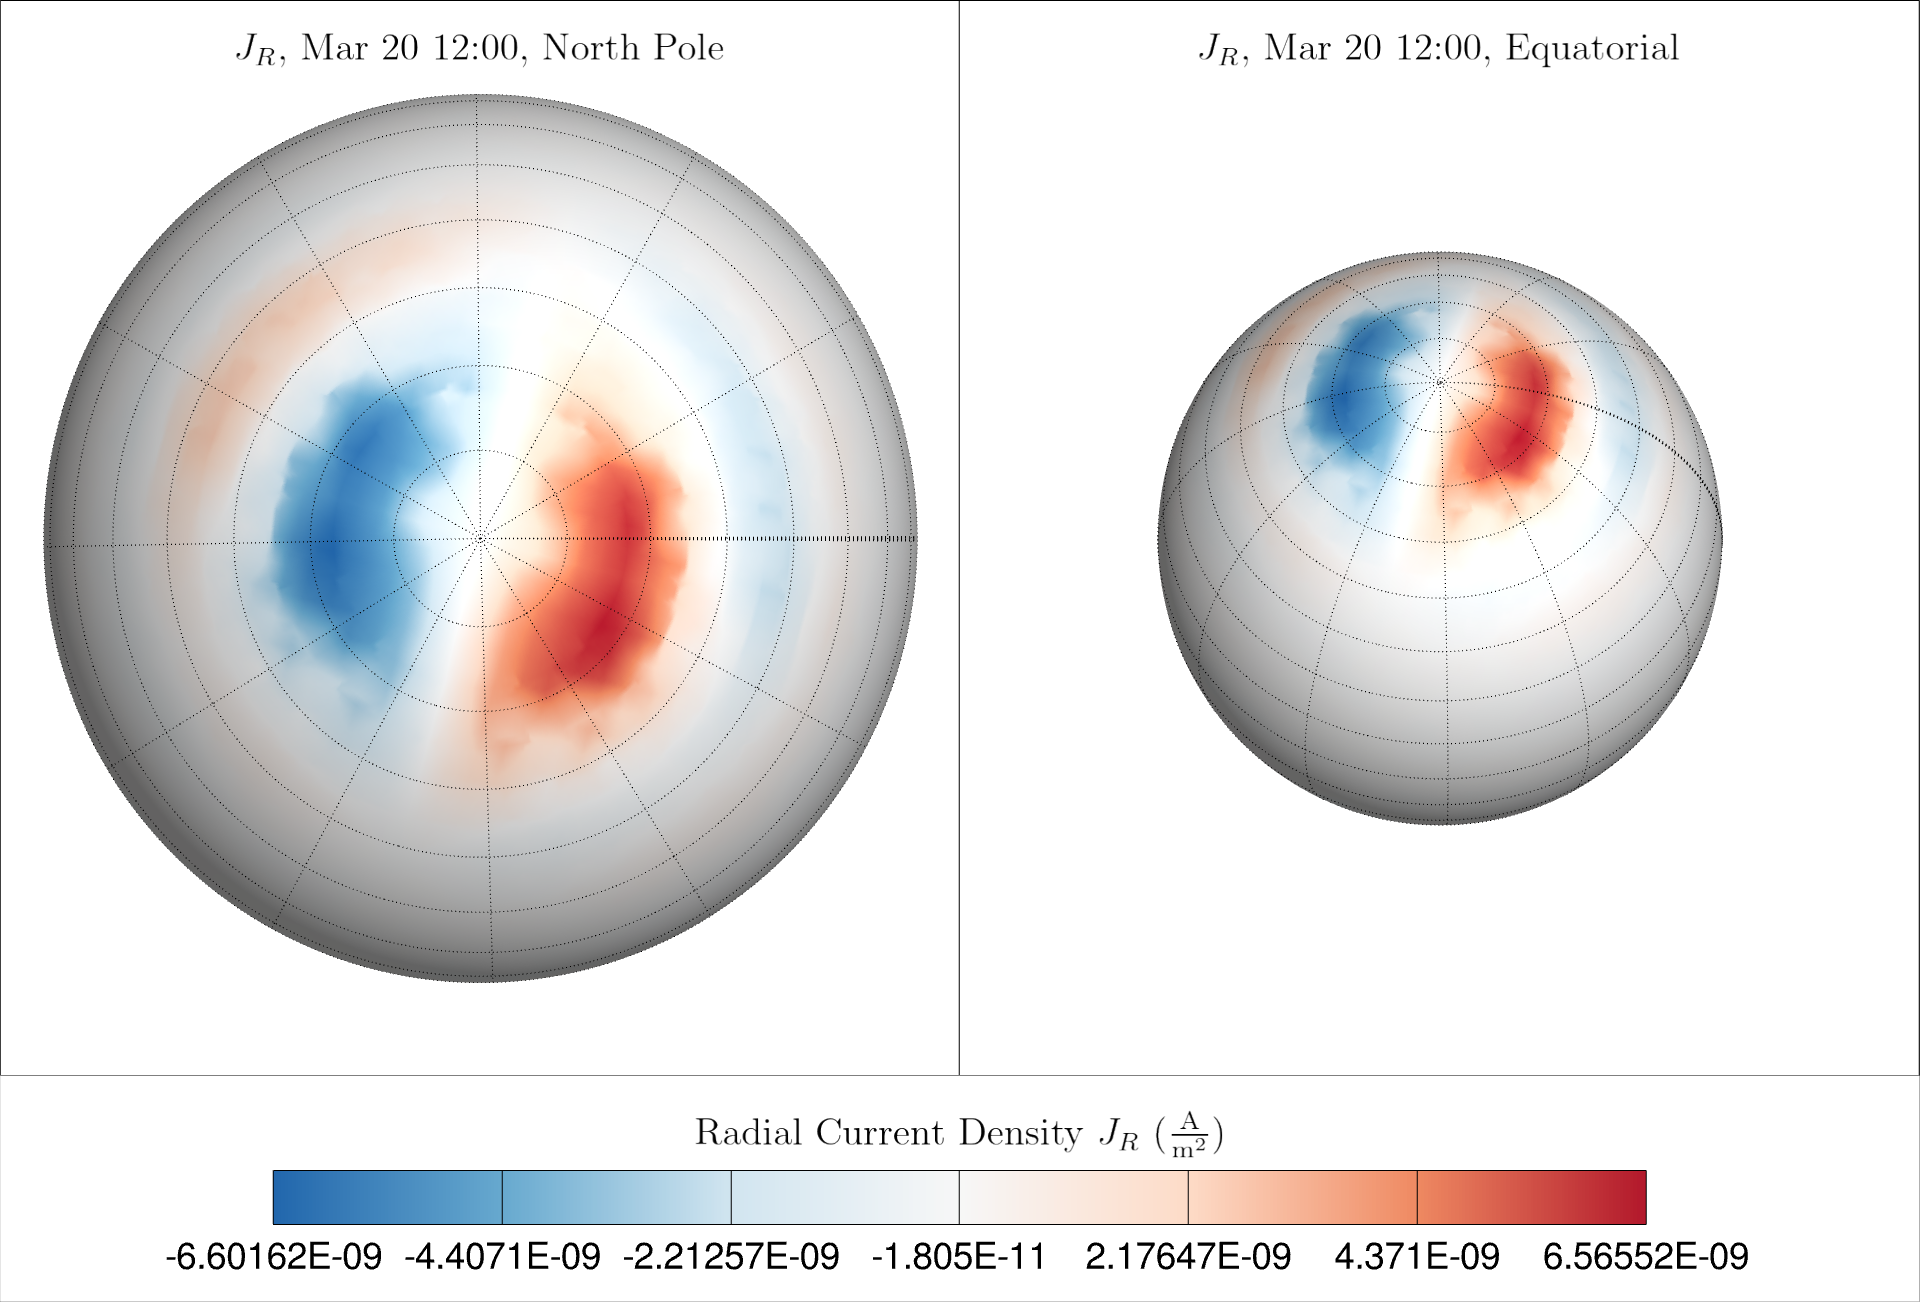
\includegraphics[width=0.67\textwidth]{figures/soureTerm.png}
	\caption{Radial current density $J_R$ ($\mathrm{A/m^2}$) at equinox (Mar 20, 12:00), showing the field-aligned current source term that drives the ionospheric electric potentials.}
	\label{fig:sourceTerm}
\end{figure}

\section{Geomagnetic Variation}
The $K_p$ index is a standardized index used to monitor geomagnetic disturbances on a global scale. It is calculated as the mean of observations from 13 contributing sub-auroral geomagnetic observatories. This is used to categorize the magnitude of geomagnetic disturbance and its irregularity into a quasi-logarithmic scale~\citep{matzka}. Figure~\ref{fig:potentialVsKp} shows the effect of increasing $K_p$ indices on the potential distribution of the ionosphere.
\begin{figure}[htbp]
	\centering
	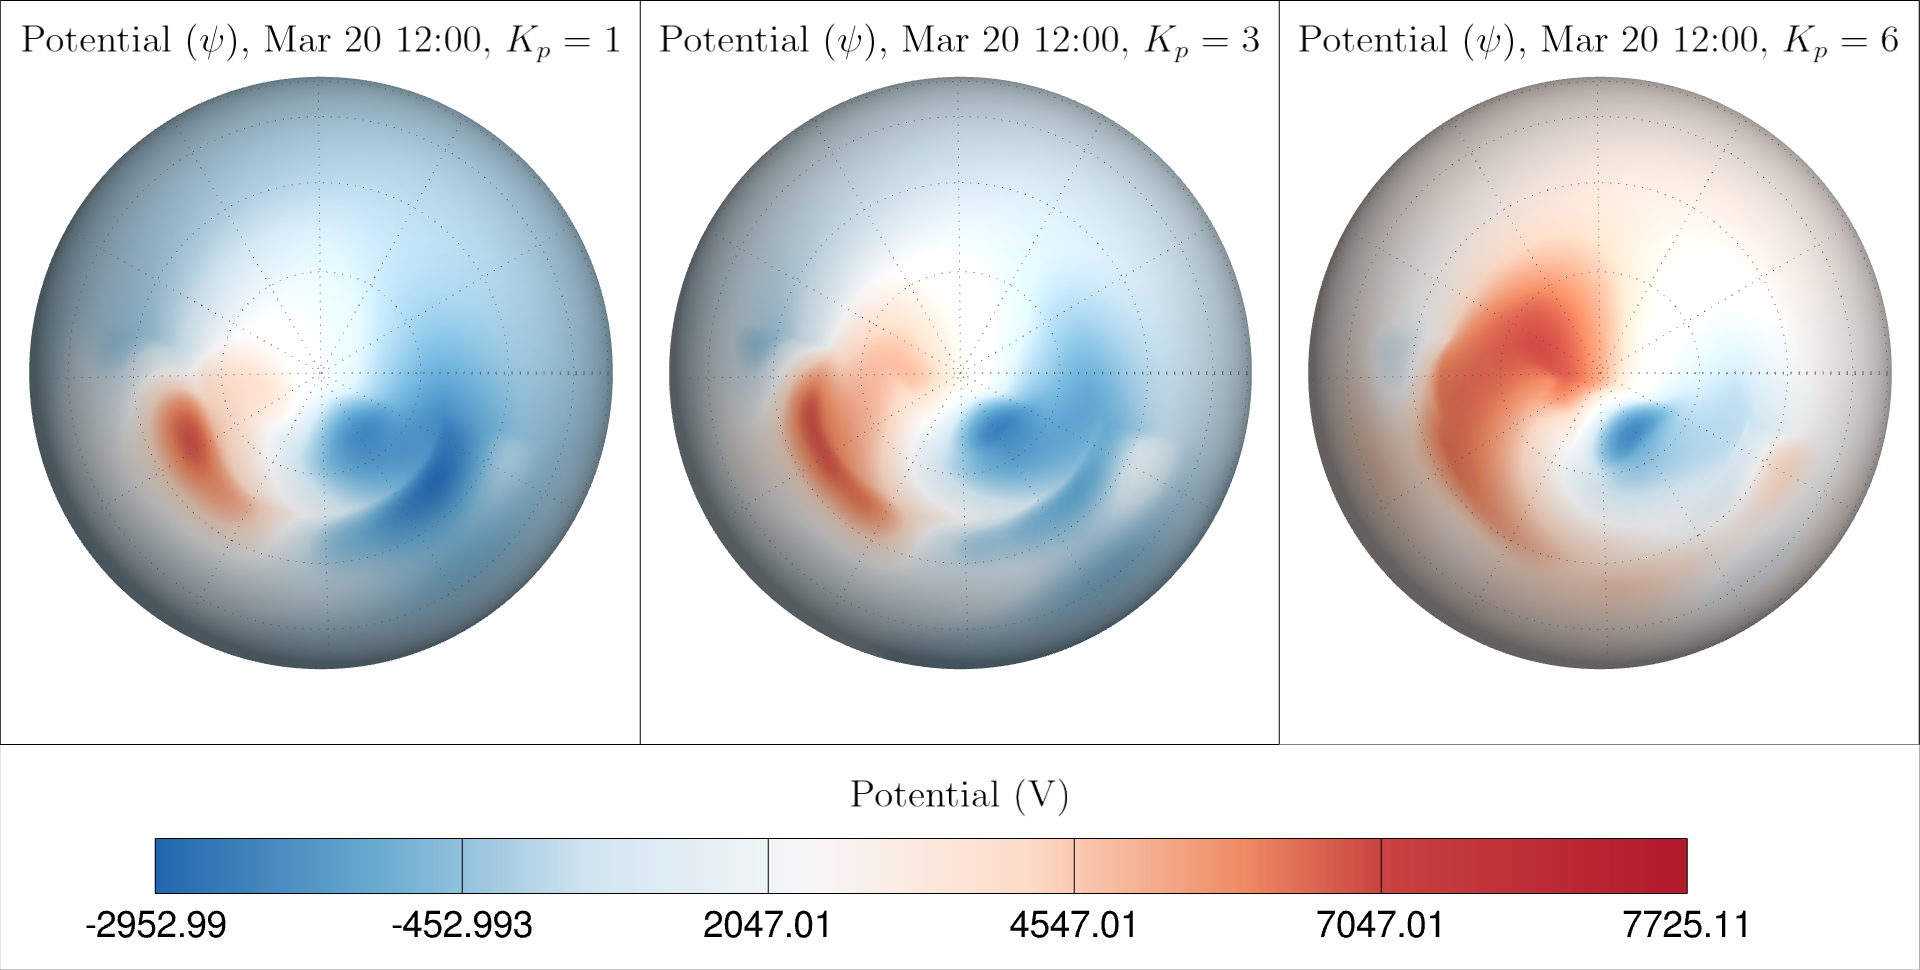
\includegraphics[width=\textwidth]{figures/potentialVsKp.png}
	\caption{Electric potential $\psi$ at the North Pole for $K_p = 1$, $3$, and $6$ at equinox (Mar 20, 12:00), showing the increasing size of the convection cells.}
	\label{fig:potentialVsKp}
\end{figure}
As shown in Figure~\ref{fig:auroralPedersonVsKp}, higher $K_p$ values generally correspond with a larger region affected by auroral precipitation. Figure~\ref{fig:potentialVsKp} shows the resulting two-cell pattern that is consistent with a southward IMF~\citep{kelley2009}. The higher $K_p$ values show a much more spread out structure for the convection cells. Conversely, in the low $K_p$ case the cells cover a significantly smaller region. During periods of high geomagnetic activity, this will result in the ionospheric currents affecting infrastructure at lower latitudes.
\section{Seasonal Variation}
\begin{figure}[H]
	\centering
	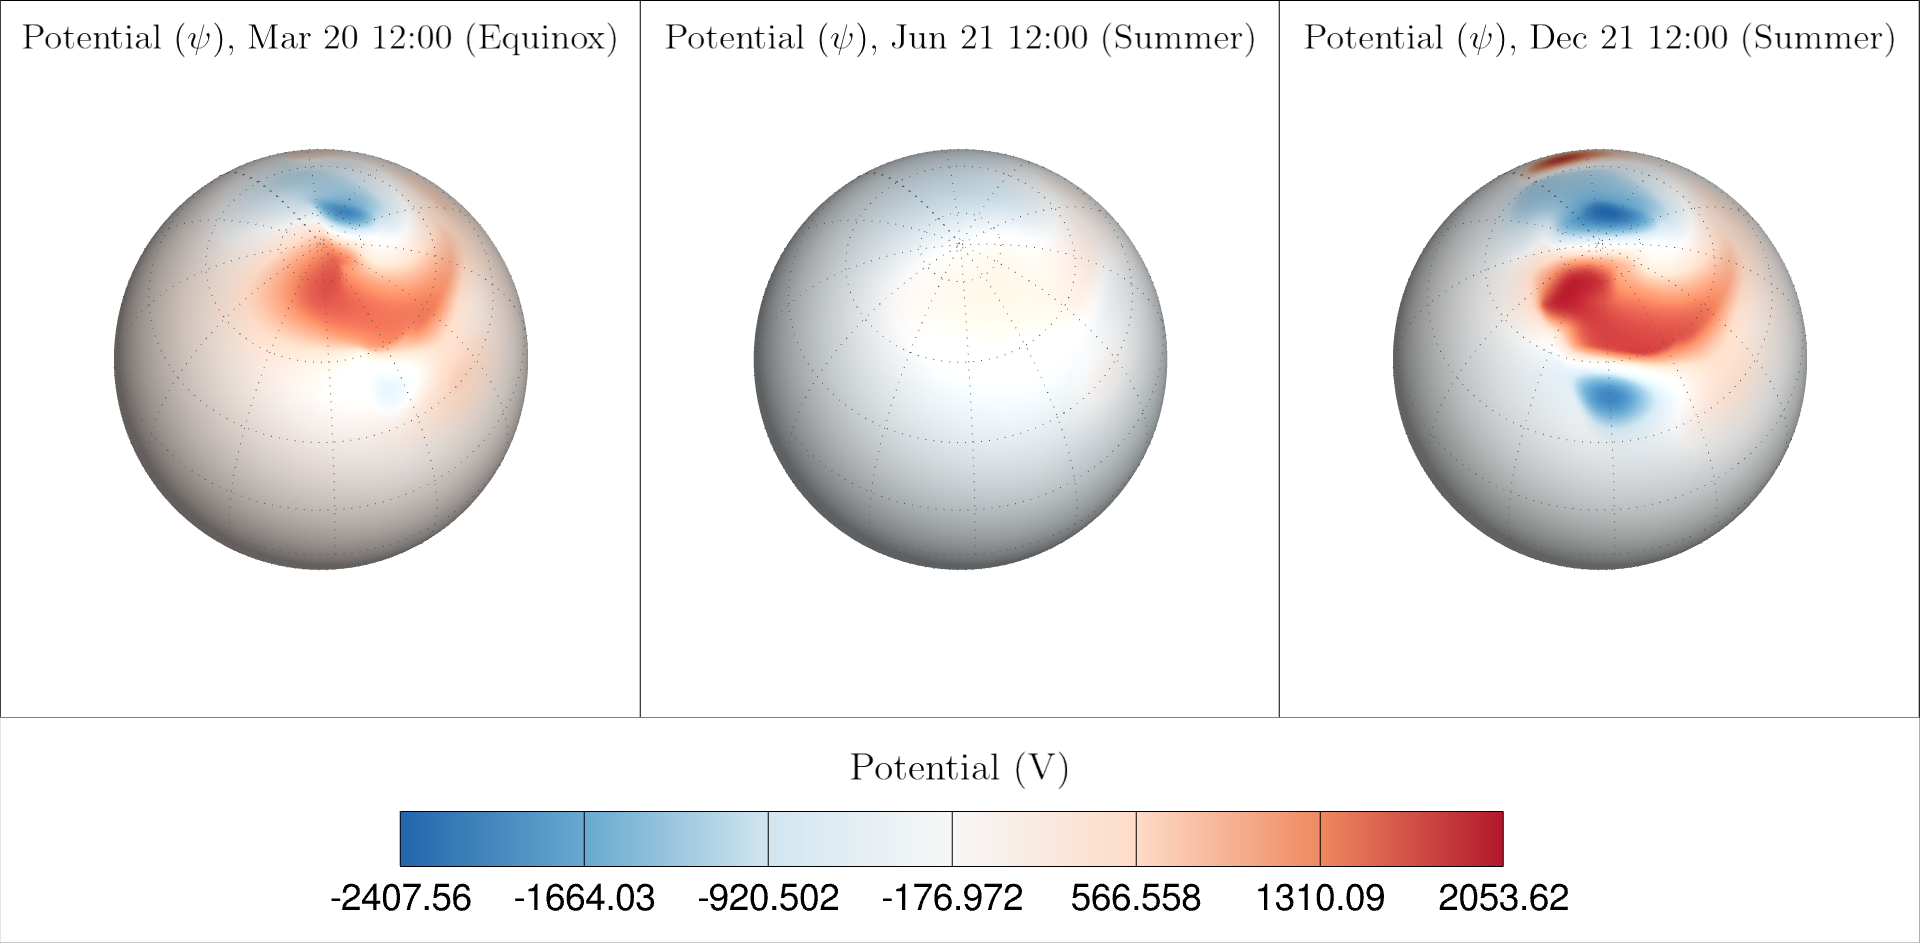
\includegraphics[width=\textwidth]{figures/potentialVsSeason.png}
	\caption{Electric potential $\psi$ at the North Pole for equinox (Mar 20), summer (Jun 21), and winter (Dec 21) at 12:00 UT, showing the seasonal effect on the intensity of the convection cells.}
	\label{fig:potentialVsSeason}
\end{figure}
Through the seasonal dependence of the conductivity discussed in Section~\ref{sec:euv_conductivity}, it is possible to analyse the behaviour of the potential solution over differing seasons. Figure~\ref{fig:potentialVsSeason} displays the seasonal variation of the potential for a spring equinox, northern-summer and northern-winter date. The varying conductivity due to sun inclination has a major effect on the intensity of the ionospheric convection cells.
\begin{figure}[H]
	\centering
	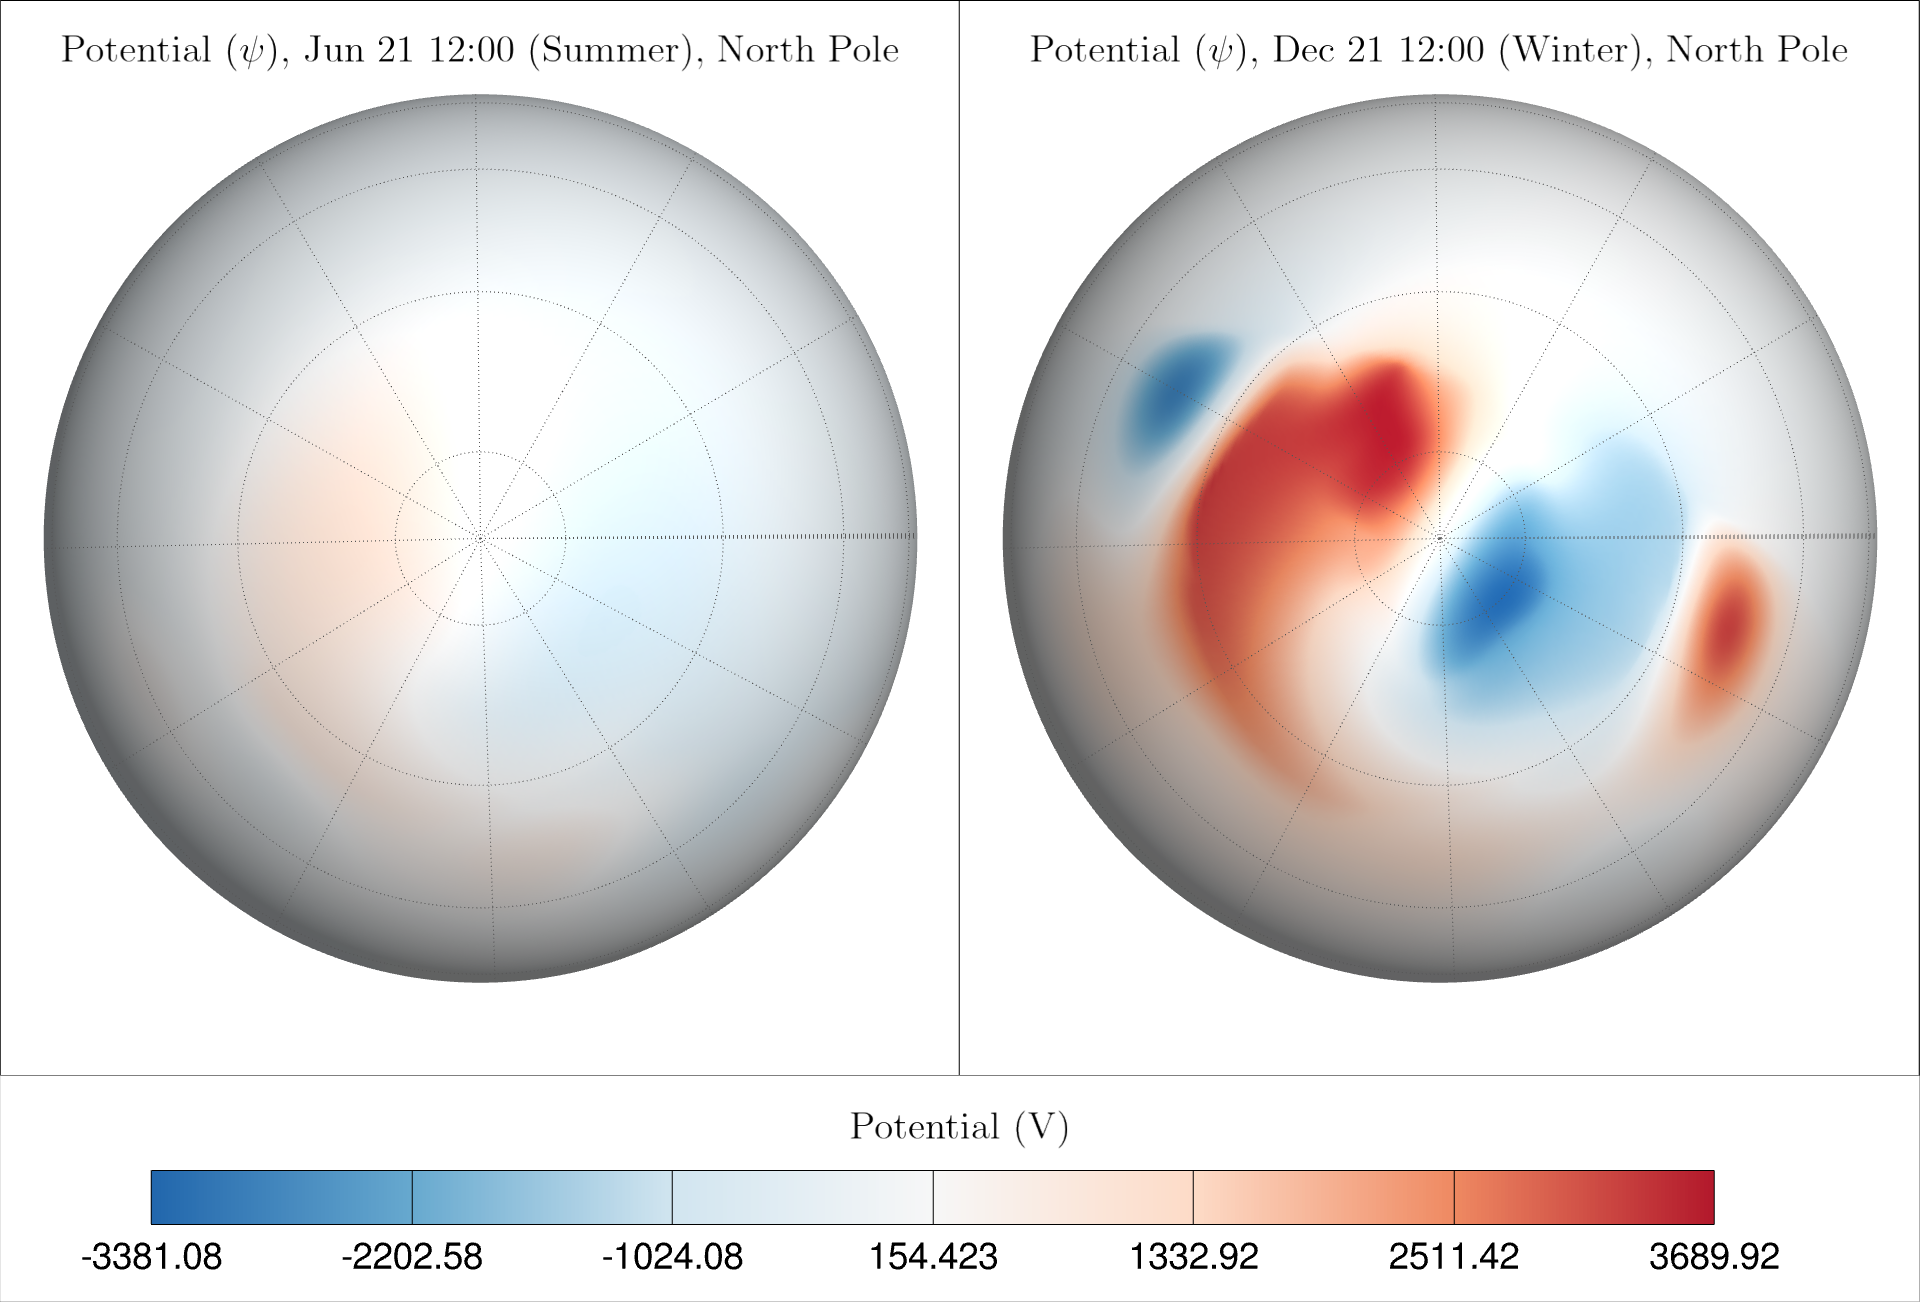
\includegraphics[width=.67\textwidth]{figures/potentialVsSeasonPole.png}
	\caption{Electric potential $\psi$ at the North Pole for summer (Jun 21), and winter (Dec 21) at 12:00 UT, showing the seasonal effect on the intensity of the convection cells.}
	\label{fig:potentialVsSeasonPole}
\end{figure}
Figure~\ref{fig:potentialVsSeasonPole} provides a clear display of the large differences that appear seasonally as viewed from above the north pole. As shown in Figure~\ref{fig:euvPedersonVsSeason}, the summer months represent a significantly higher level of conductance due to EUV ionization in the north pole. Due to this, the currents do not dissipate as much energy through the north pole convection cells. These results show that winter months can result in higher potential gradients in high latitude regions, increasing the probability of adverse interference with ground based infrastructure.
\begin{figure}[H]
	\centering
	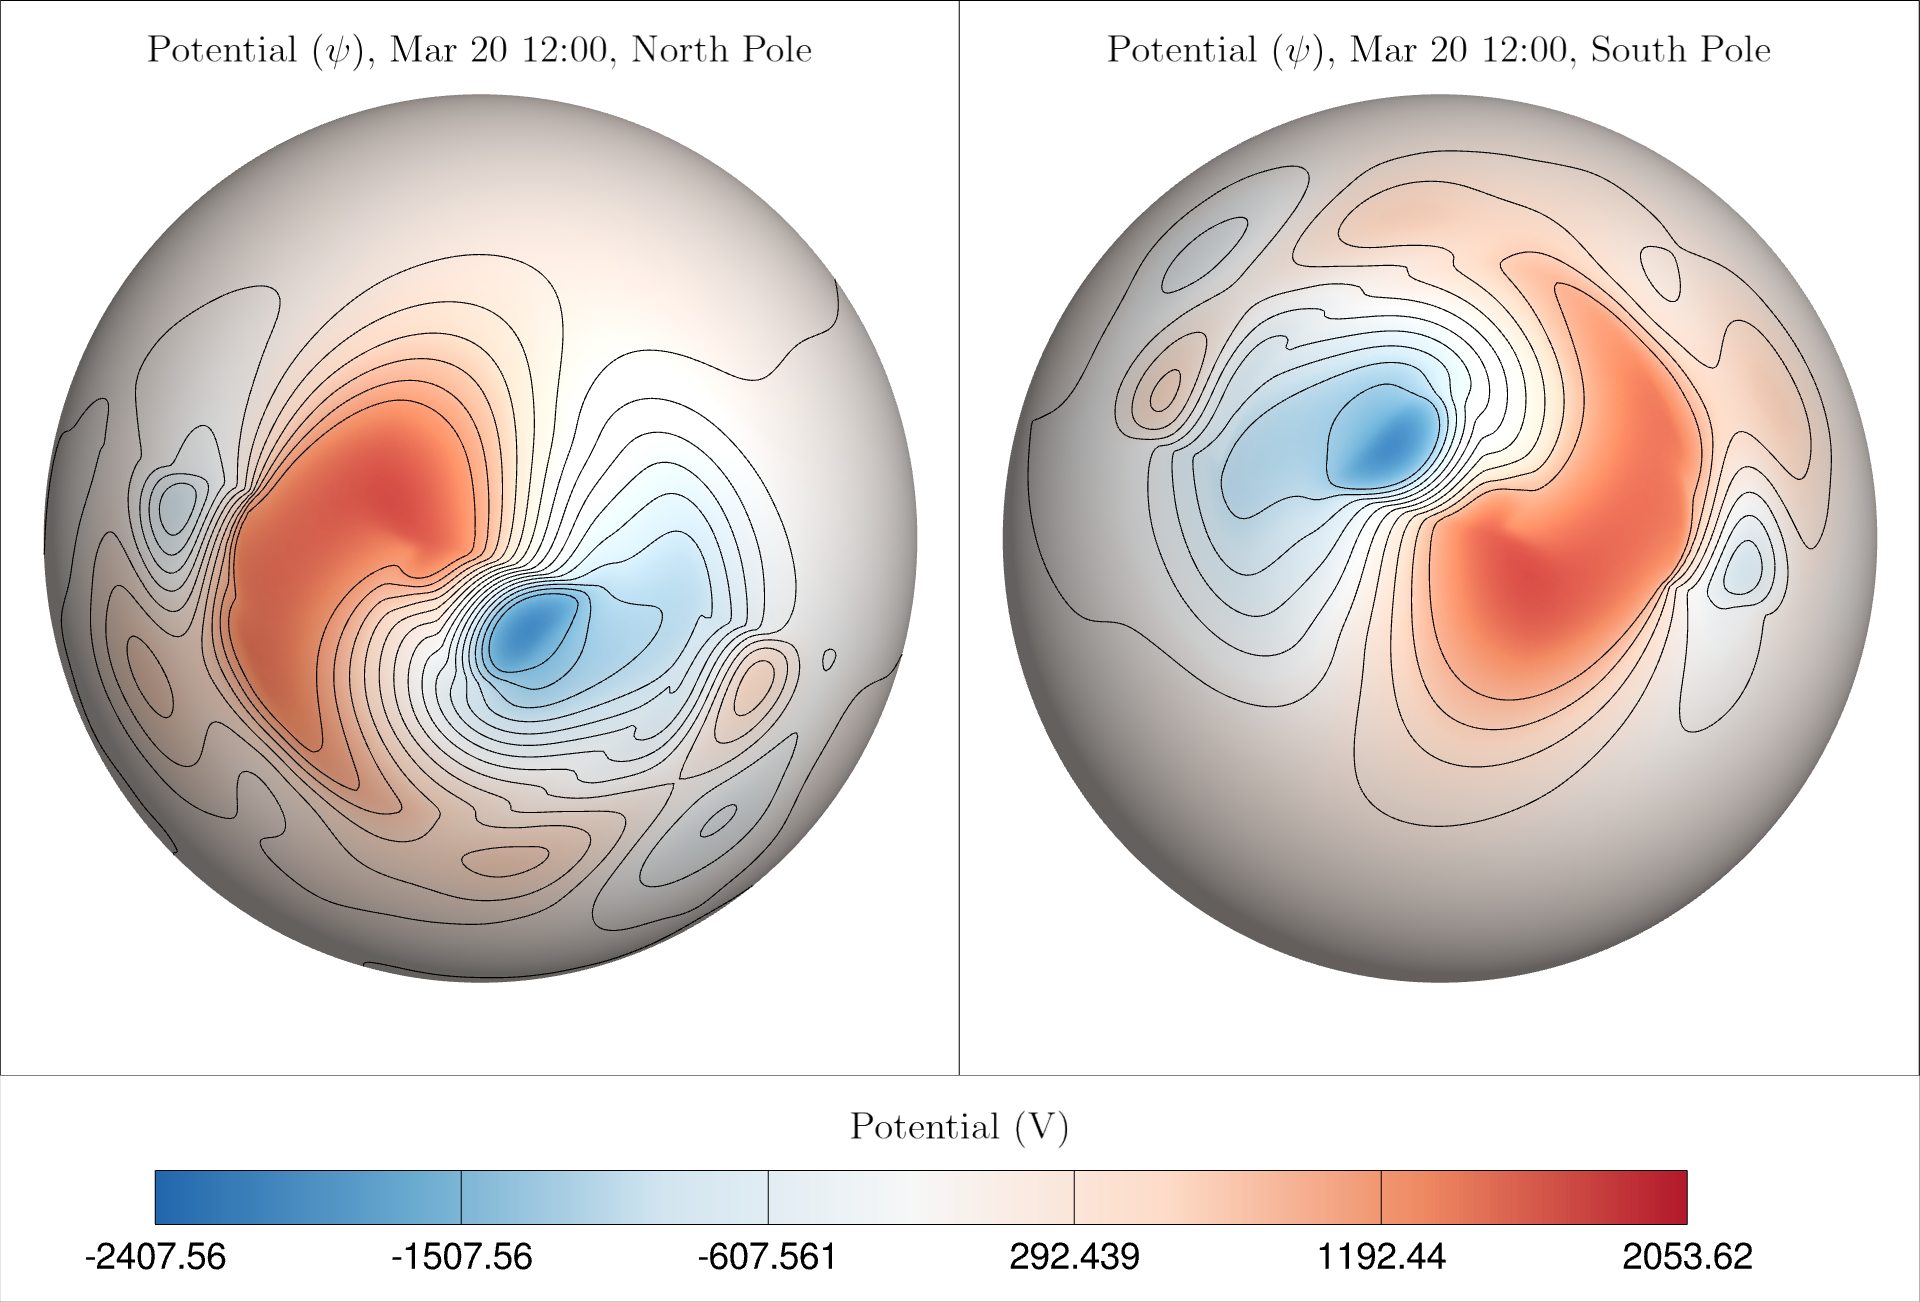
\includegraphics[width=\textwidth]{figures/poleContours.png}
	\caption{Electric potential $\psi$ at the north and south pole for equinox (Mar 20) conditions. Contour lines overlaid to show the continuity of the boundary condition.}
	\label{fig:boundaryCondition}
\end{figure}
These results exhibit clear continuous boundary behaviour at the poles (Figure~\ref{fig:boundaryCondition}) while showing a clear two-cell pattern that is characteristic of a southward IMF~\citep{kelley2009}. This qualitative analysis shows that the model obeys behaviour consistent with the known behaviour of the ionosphere. More robust verification of the model's predictions will become possible with the completion of the magnetosphere-ionosphere coupling procedure, allowing for a comprehensive study of varied radial current data.
